\documentclass{ctexart}
\usepackage{babel}
\usepackage{anyfontsize}
\usepackage[letterpaper,top=2cm,bottom=2cm,left=3cm,right=3cm,marginparwidth=1.75cm]{geometry}
\usepackage{amsmath, amssymb}
\usepackage{graphicx}
\usepackage{floatrow}
\usepackage[colorlinks=true, allcolors=blue]{hyperref}
\usepackage{enumitem}
\usepackage{longtable}
\usepackage{listings}
\usepackage{xcolor}
\definecolor{teal}{RGB}{0,128,128}
\setlist[itemize]{noitemsep}
\lstset{
    basicstyle          =   \sffamily,          % 基本代码风格
    keywordstyle        =   \bfseries,          % 关键字风格
    commentstyle        =   \rmfamily\itshape,  % 注释的风格,斜体
    stringstyle         =   \ttfamily,  % 字符串风格
    flexiblecolumns,                % 别问为什么,加上这个
    numbers             =   left,   % 行号的位置在左边
    showspaces          =   false,  % 是否显示空格,显示了有点乱,所以不现实了
    numberstyle         =   \zihao{-5}\ttfamily,    % 行号的样式,小五号,tt等宽字体
    showstringspaces    =   false,
    captionpos          =   t,      % 这段代码的名字所呈现的位置,t指的是top上面
    frame               =   lrtb,   % 显示边框
}

\lstdefinestyle{Python}{
    language        =   Python, % 语言选Python
    basicstyle      =   \zihao{-5}\ttfamily,
    numberstyle     =   \zihao{-5}\ttfamily,
    keywordstyle    =   \color{blue},
    keywordstyle    =   [2] \color{teal},
    stringstyle     =   \color{magenta},
    commentstyle    =   \color{red}\ttfamily,
    breaklines      =   true,   % 自动换行,建议不要写太长的行
    columns         =   fixed,  % 如果不加这一句,字间距就不固定,很丑,必须加
    basewidth       =   0.5em,
}

\title{\textbf{数据科学导论实验报告}}
\author{吕思翰\ 来泽远\ 曹宸瑞}

\begin{document}

\maketitle

% \tableofcontents
% \newpage

% \ctexset{abstractname=摘要}
% \begin{abstract}

% \end{abstract}

\section{比赛名称}

Predict CO2 Emissions in Rwanda(预测卢旺达二氧化碳排放量)

\section{成员}

\begin{itemize}
      \item 吕思翰 PB21000144
      \item 来泽远 PB21000164
      \item 曹宸瑞 PB21020659
\end{itemize}

\section{问题定义}

\subsection{Predicting CO2 Emissions}

准确监测碳排放能力是应对气候变化的重要步骤。精确的碳排放数据使研究人员和政府能够了解碳排放的来源和模式。尽管欧洲和北美已经建立了广泛的地面碳排放监测系统,但在非洲可用的系统相对较少。本任务要求参赛选手依据过往二氧化碳排放数据预测未来的排放数据。

\subsection{Dataset}

从卢旺达多个地区挑选了大约497个独特的地点,分布在农田、城市和发电厂周围。这次比赛的数据是按时间划分的;训练数据中包含2019 - 2021年的二氧化碳排放数据,任务是预测2022年至11月的二氧化碳排放数据。

\subsection{Evaluation}

本次比赛的评价指标是均方根误差(RMSE)。RMSE是预测值和实际值之间差异的平方的平均值的平方根。RMSE的值越低,表示模型的预测能力越好。RMSE定义为:

\[
    RMSE=\sqrt{\frac{1}{N}\sum\limits_{i=1}^{N}(y_i-\hat y_i)^2}.
\]

其中 $y_i$ 是真实值,$\hat y_i$ 是预测值,$N$ 是样本数量。

\section{数据分析}

\subsection{数据概览与特性}

\begin{table}[h]
      \centering
      \begin{tabular}{l|l|l|l}
      \hline
          \ & Column & Non-Null Count & Dtype \\ \hline
          0 & \texttt{ID\_LAT\_LON\_YEAR\_WEEK} & 79023 \texttt{non-null} &
          \texttt{object} \\
          1 & \texttt{latitude} & 79023 \texttt{non-null} & \texttt{float64} \\
          2 & \texttt{longitude} & 79023 \texttt{non-null} & \texttt{float64} \\
          3 & \texttt{year} & 79023 \texttt{non-null} & \texttt{int64} \\
          4 & \texttt{week\_no} & 79023 \texttt{non-null} & \texttt{int64} \\
          5 & \texttt{SulphurDioxide\_SO2\_column\_number\_density} & 64414
          \texttt{non-null} & \texttt{float64} \\
          6 & \texttt{SulphurDioxide\_SO2\_column\_number\_density\_amf} & 64414
          \texttt{non-null} & \texttt{float64} \\
          \ldots{} & & & \\
          74 & \texttt{Cloud\_solar\_zenith\_angle} & 78539 \texttt{non-null} &
          \texttt{float64} \\
          75 & \texttt{emission} & 79023 \texttt{non-null} & \texttt{float64} \\
          \hline
      \end{tabular}
      \caption{数据集概览}
\end{table}

\begin{itemize}
      \item 数据集共有79023行,76列,其中75列为特征,1列为预测值。
      \item 除经纬度外其余值均为 \texttt{float64},不需要做额外数据处理。
      \item 部分测试量包含空值,可以进行缺失值处理。
      \item 可用作索引的值有 \texttt{latitude},\texttt{longitude},\texttt{year} \texttt{week\_no},需预测值为 \texttt{emission}
      \item 其余特征可以分类为 \texttt{CarbonMonoxide},\texttt{Cloud}, \texttt{Formaldehyde},\texttt{NitrogenDioxide},\texttt{Ozone},\texttt{SulphurDioxide},\texttt{UvAerosolIndex},\texttt{UvAerosolLayerHeight}。
\end{itemize}

\subsection{特征分析}

\subsubsection{年份与周数}

首先我们考虑排放量与时间的关系。我们将年份和周数相关联作为日期,作出总排放量关于日期的折线图,得到结果如下(红线划分了2019-2021年的数据):

\begin{figure}[H]
      \centering
      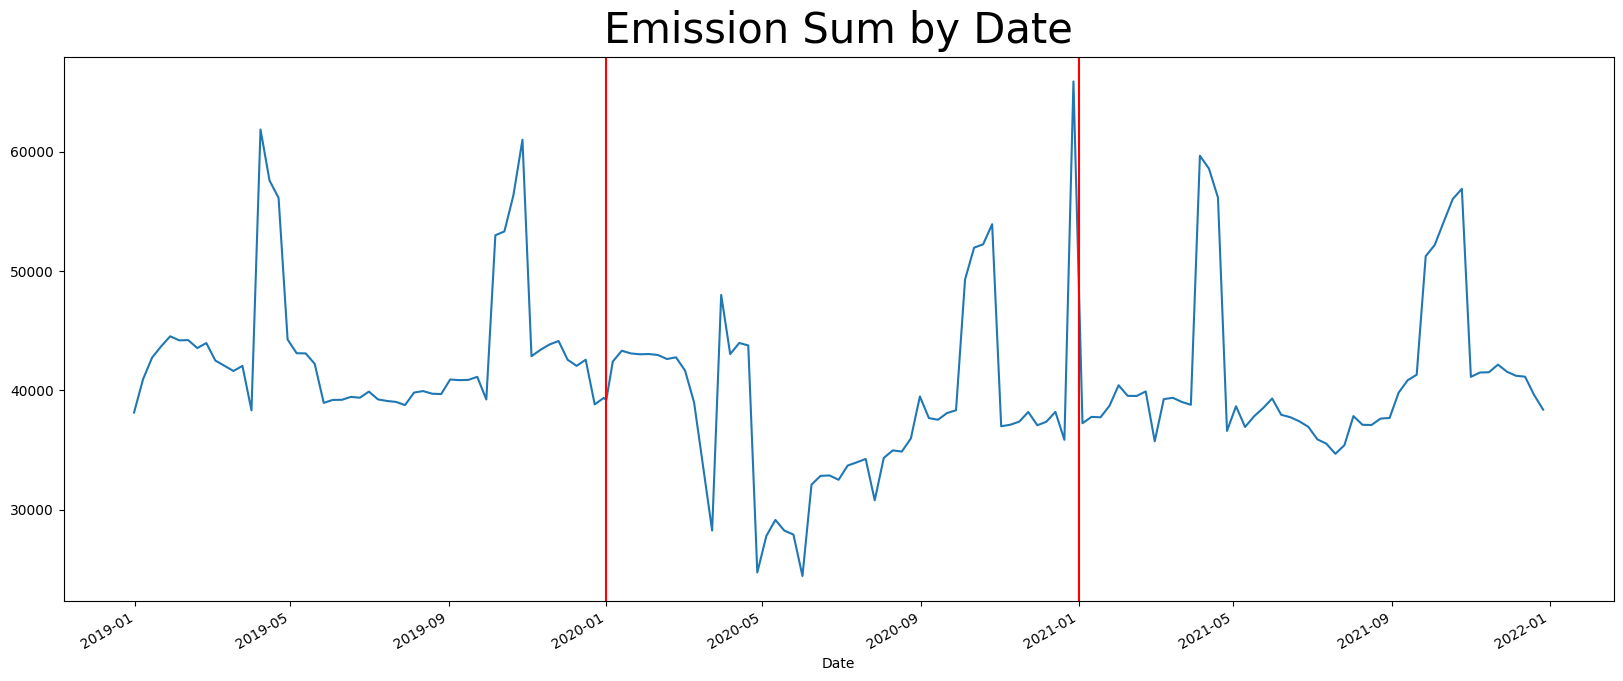
\includegraphics[width=1\textwidth]{output2.png}
      \caption{date与emission的折线图}
\end{figure}

可以看出,排放量随时间的变化呈现出一定的周期性,因此我们认为年份和周数对于预测二氧化碳排放量有一定的参考价值。我们将年份和周数作为特征之一加入模型。

但是,值得注意的是,由于新冠病毒的影响,2020年的数据与其他年份的数据有较大的差异,后续需要针对2020年的数据进行特殊处理。

我们将2019与2021年的数据平均后,作图得到排放量关于月份的折线图,结果如下:

\begin{figure}[H]
      \centering
      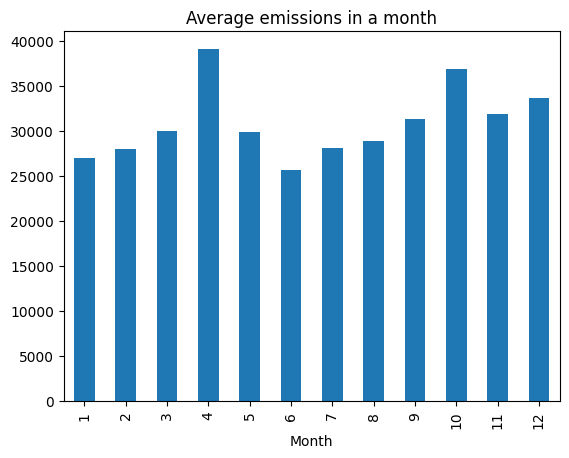
\includegraphics[width=0.6\textwidth]{output3.png}
      \caption{排放量关于月份的折线图}
\end{figure}

结合两图可以发现,一年内某几个特殊的月份具有较高的排放量,这可能与人类生产活动习惯相关。对于同一个地点,周数(月份)与排放量具有较高的相关性,且关于年份呈现周期变化。这对于数据处理有一定的借鉴意义。

\subsubsection{经纬度}

首先,我们将每个地区的排放量求和,以其排放量为半径,以其经纬度为圆心,按照排放量高低标记颜色从浅至深,作出排放量关于经纬度的分布图,结果如下:

\begin{figure}[H]
      \centering
      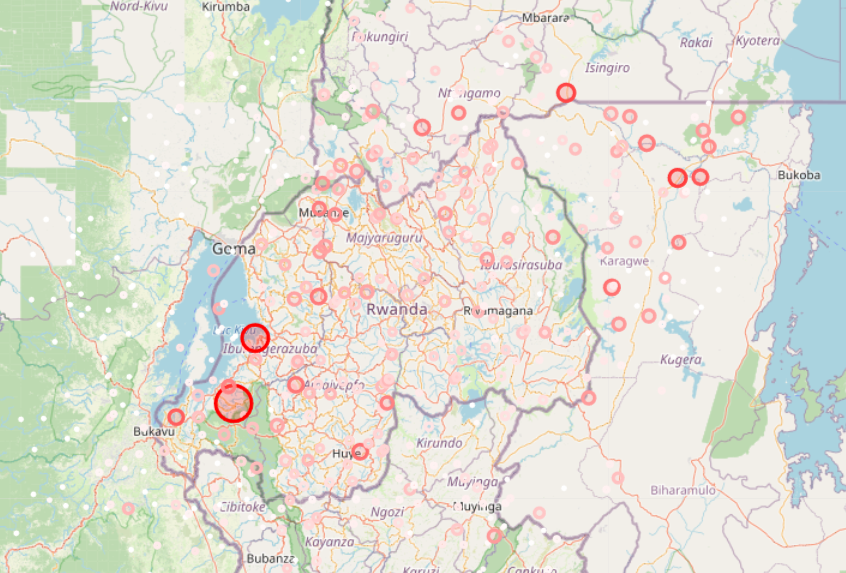
\includegraphics[width=0.8\textwidth]{output4.png}
      \caption{排放量关于经纬度的分布图}
\end{figure}

和城市聚集类似,几个距离较近的采样点,他们的碳排放量也是相近的,并且不难发现大部分采样点较为密集,这为使用聚类提供了数据支持。在模型中,可以使用距离相近的采样点的数据来相互预测。

其次,我们考察不同地点碳排放的变化,作出各地点以年为单位的碳排放量变化如图\ref{fig:5}:

\begin{figure}[H]
      \centering
      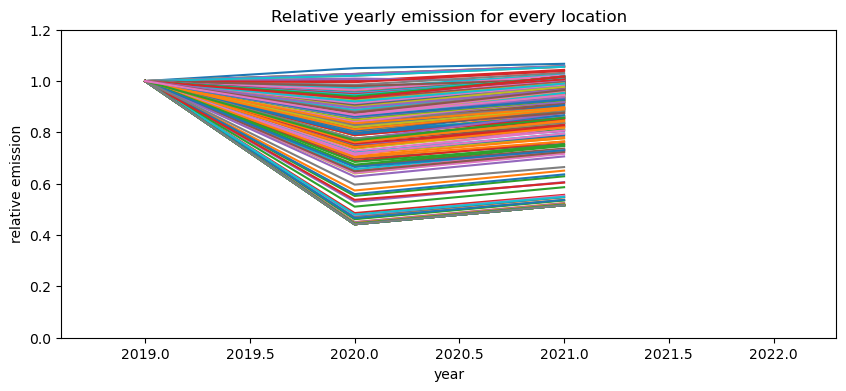
\includegraphics[width=0.8\textwidth]{output5.png}
      \caption{\label{fig:5}各地点排放量关于年份的折线图}
\end{figure}

我们将每一年的碳排放除以2019年的碳排放,作为相对值。若排除新冠的影响,对于绝大部分地点,其碳排放是较为稳定的,在某一个基准附近存一定浮动(多为上升)。而对于这个基准值,经纬度是与其强相关的。

\subsubsection{关于时间和空间的总结}

作出各个地点以周为单位的碳排放量图以及相对变化量如下:

\begin{figure}[H]
      \centering
      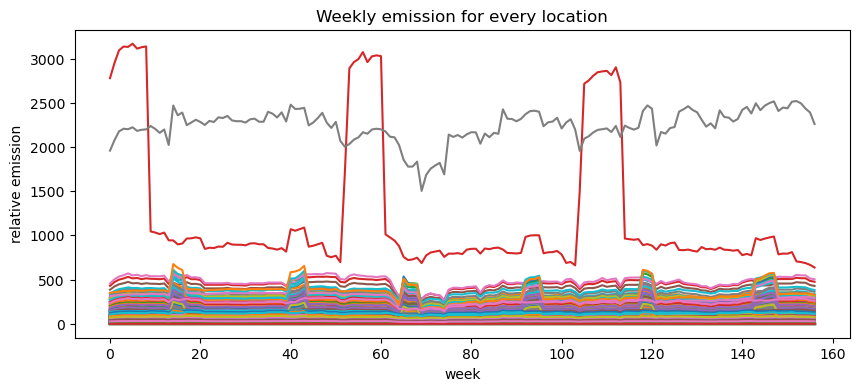
\includegraphics[width=0.8\textwidth]{output8.png}
      \caption{各地点排放量关于周数的折线图}
\end{figure}

\begin{figure}[H]
      \centering
      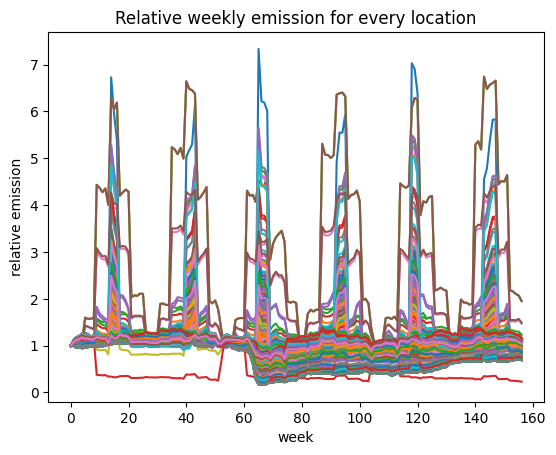
\includegraphics[width=0.8\textwidth]{output6.png}
      \caption{排放量相对变化量}
\end{figure}

建模可以大致从以下方面入手:

\subsubsection{其他特征}

除了上述特征外,数据集还给出了大量的气象数据,包括二氧化硫(SO2)、一氧化碳(CO)、二氧化氮(NO2)、甲醛(HCHO)、臭氧(O3)、紫外线气溶胶、云等物质的方位角、天顶角、深度、角度、密度、压力、温度、反射率等信息。我们认为这些信息对于预测二氧化碳排放量有一定的参考价值。以下是对这些特征的分析。

以2020年 \texttt{SulphurDioxide\_SO2\_column\_number\_density} 为例,计算其与 \texttt{emission} 的相关系数并作出散点图,代码如下:

\begin{lstlisting}[style=Python]
      # 加载数据
      data_path = os.path.abspath('.') + '/../data/'
      df = pd.read_csv(data_path + "train.csv")
      col = "SulphurDioxide_SO2_column_number_density"
      df = df[df['year'] == 2020]
      df = df.dropna(subset=[col, 'emission'])
      
      # 计算相关系数
      pearson_corr, _ = pearsonr(df[col], df['emission'])
      spearman_corr, _ = spearmanr(df[col], df['emission'])
      
      # 绘制散点图
      plt.figure(figsize=(10, 6))
      sns.scatterplot(x=col, y='emission', data=df)
      plt.title('Scatter plot of ' + col + ' vs emission')
      plt.show()
      
      # 进行回归分析
      X = sm.add_constant(df[col])
      model = sm.OLS(df['emission'], X)
      results = model.fit()
\end{lstlisting}

得到结果如下:

\begin{center}
Pearson correlation: -0.013960940599134839

Spearman correlation: -0.06904123013729443
\end{center}


\begin{figure}[H]
      \centering
      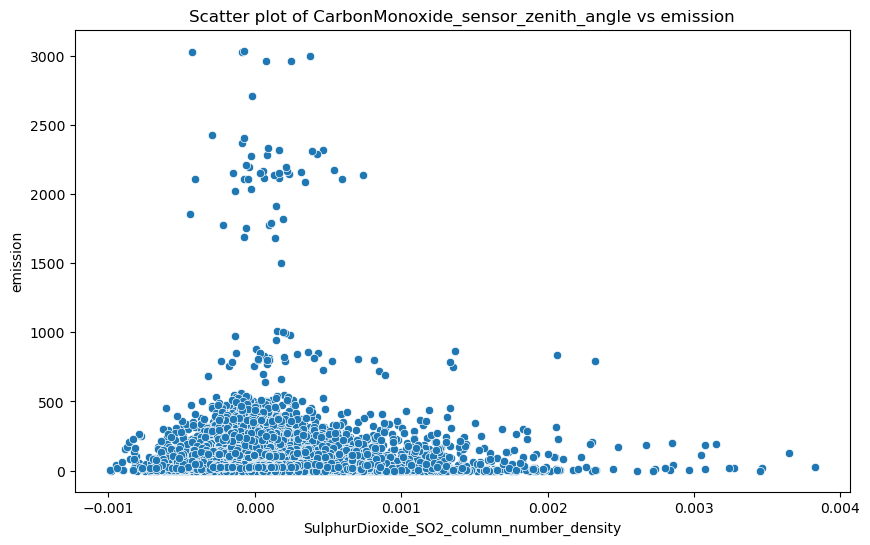
\includegraphics[width=0.8\textwidth]{output1.png}
      \caption{\texttt{SulphurDioxide\_SO2\_column\_number\_density} 与 \texttt{emission} 的散点图}
\end{figure}

可以看出,这两者之间的相关性非常小,因此我们认为\texttt{SO2\_column\_number\_density}数据对于预测二氧化碳排放量的影响可以忽略不计。

我们还对其他气象数据进行了类似的分析,没有出现与CO2有较大相关性的数据。初步分析后,我们认为这些气象数据与CO2排放量之间可能没有明显关系,理由如下:

\begin{itemize}
      \item 卢旺达是一个直径200公里的小国,每天都有邻国的空气取代卢旺达的整个大气。即使卢旺达所产生的各种气体之间有一定的相关性,也会被邻国的空气所影响。
      \item 二氧化碳排放来自不同的部门(地面交通、空中交通、供暖、发电、工厂等),而这些部门并不一定排放与CO2成比例的NO2、CO、SO2等气体。我们认为只在特定区域如工厂,CO2可能会与S02等成正比例关系。
\end{itemize}

因此,我们借用排放量地图进行分析,对排放量最多的地点测量得到的数据进行相关性分析。有理由相信如果CO2主要来自工厂,会同时产生大量SO2、CO等气体。以2021年CarbonMonoxide CO column number density为例,得到结果如下:

\begin{center}
      Pearson correlation: -0.0016211411671317282

      Spearman correlation: 0.002390506275078972
\end{center}

\begin{figure}[H]
      \centering
      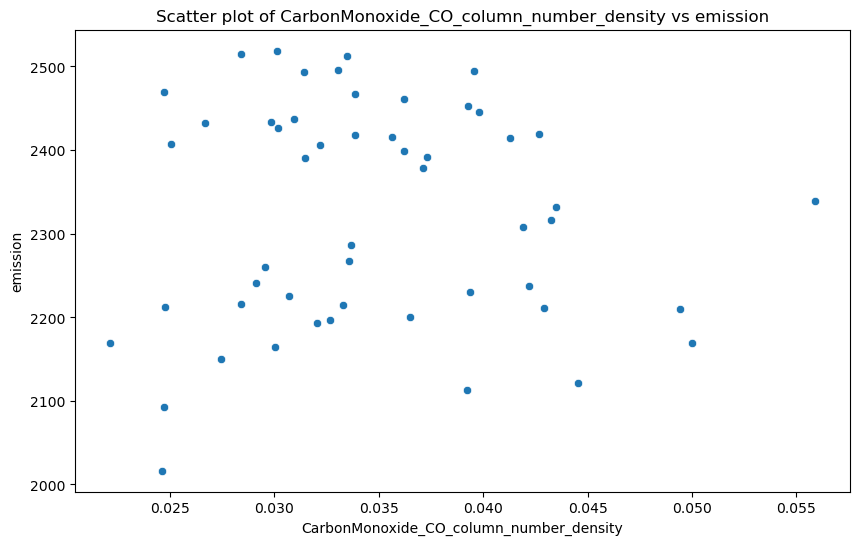
\includegraphics[width=0.8\textwidth]{output7.png}
      \caption{\texttt{CarbonMonoxide\_CO\_column\_number\_density} 与 \texttt{emission} 的散点图}
\end{figure}

我们无法得出该气体与CO2排放量之间有明显的相关性。类似的,我们对该地点的其他气象数据进行了计算,也未能分析出得到更多有价值的信息。

Ozone\_solar\_azimuth\_angle

% \subsubsection{权重量化}

\subsection{数据预处理}

\subsubsection{缺失值处理}

在数据预处理阶段,缺失值处理是一个重要的步骤。缺失值可能会导致统计分析的结果出现偏差,或者使得机器学习算法无法正确地工作。

使用\verb|train.isnull().sum()|可以查看训练集每一列的缺失值数量,结果如表\ref{tab:1}所示。

\begin{table}[h]
      \centering
      \begin{tabular}{l|l}
      \hline
      Column & Non-Null Count \\ \hline
      \texttt{UvAerosolLayerHeight\_aerosol\_height} & 78584 \\
      \texttt{UvAerosolLayerHeight\_solar\_zenith\_angle} & 78584 \\
      \texttt{UvAerosolLayerHeight\_solar\_azimuth\_angle} & 78584 \\
      \ldots{} & \\
      \texttt{NitrogenDioxide\_tropopause\_pressure} & 18320 \\
      \texttt{NitrogenDioxide\_stratospheric\_NO2\_column\_number\_density} & 18320 \\
      \texttt{NitrogenDioxide\_NO2\_slant\_column\_number\_density} & 18320 \\
      \ldots{} & \\
      \texttt{SulphurDioxide\_SO2\_column\_number\_density\_15km} & 14609 \\
      \texttt{SulphurDioxide\_solar\_zenith\_angle} & 14609 \\
      \texttt{SulphurDioxide\_solar\_azimuth\_angle} & 14609 \\
      \ldots{} & \\
      \hline
      \end{tabular}
      \caption{\label{tab:1}缺失值概览}
\end{table}

虽然某些机器学习算法,如决策树和随机森林,可以直接处理缺失值,但由于后续模型还未确定,故还是在此对缺失值进行处理。对于缺失值较多的列,如\texttt{UvAerosolLayerHeight},缺失率达到99\%,我们可以考虑直接删除。对于缺失值较少的列,我们可以考虑使用均值填充。

对于测试集,我们可以进行类似缺失值处理操作。

\subsubsection{数据归一化}

数据归一化是一种常用的数据预处理技术,用于将数据转换到一个公共的尺度。这种技术在机器学习和数据挖掘中非常常见,因为许多算法(如神经网络)对输入数据的尺度和分布有一定的假设。

数据归一化通常涉及将数值特征缩放到一个固定的范围(如0到1),或者将它们转换为具有零均值和单位方差的值。这样可以确保所有特征在模型训练过程中具有相同的重要性,而不会因为它们的尺度不同而被赋予不同的权重。

可以使用 \texttt{sklearn.preprocessing} 模块中的 \texttt{MinMaxScaler} 或 \texttt{StandardScaler} 类来进行数据归一化,代码如下:

\begin{lstlisting}[style=Python]
      from sklearn.preprocessing import StandardScaler
      scaler = StandardScaler()
      train = scaler.fit_transform(train)
\end{lstlisting}

\subsection{模型选择}

这是一个回归问题,我们尝试了多种回归模型,包括线性回归、逻辑回归、支持向量回归、决策树回归、类别提升、自适应提升、极端梯度提升、随机森林、半径近邻、K近邻等。

\subsubsection{LinearRegression(线性回归)}

\subsubsection{SupportVectorRegressor(支持向量回归)}

\subsubsection{DecisionTreeRegressor(决策树回归)}

\subsubsection{CatBoostRegressor(类别提升)}

\subsubsection{AdaBoostRegressor(自适应提升)}

\subsubsection{XGBoostRegressor(极端梯度提升)}

\subsubsection{RandomForestRegressor(随机森林)}

我们使用了经纬度、年份、周数作为输入,参数设置min\_samples\_leaf=6,使用随机森林模型进行训练,得到的结果如下:

\subsubsection{RadiusNeighborsRegressor(半径近邻)}

\subsubsection{KNeighborsRegressor(K近邻)}

% \subsubsection{MLPRegressor(多层感知器)}

% \subsubsection{LGBMRegressor(LightGBM回归)}

% \subsubsection{GradientBoostingRegressor(梯度提升回归)}

\subsection{结果处理}

显然,预测出的CO2排放量不可能为负数,因此我们将预测出的负数值置为0。

除此之外,我们相信训练集的数据中,如果某个地点在2019-2021年的CO2排放量均为0,那么这个地点在2022年的CO2排放量也应该为0。因此,我们将这些地点的预测值置为0。

代码如下:

\begin{lstlisting}[style=Python]
      y_pred[y_pred < 0] = 0
      
      zero_emissions = train.groupby(['latitude', 'longitude'])['emission'].mean().to_frame()
      zero_emissions = zero_emissions[zero_emissions['emission'] == 0]
      mask = test.apply(lambda x: (x['latitude'], x['longitude']) in zero_emissions.index, axis=1)
      y_pred.loc[mask, "emission"] = 0
\end{lstlisting}

处理后对评估结果(RMSE)有一定的提升。

\section{评估}

\subsubsection{交叉验证}

\subsubsection{RMSE}

\section{团队成员分工}

\subsection{吕思翰}

\subsection{来泽远}

\subsection{曹宸瑞}

\section{总结与感悟}

\ctexset{bibname=参考文献}
\begin{thebibliography}{100}
\bibitem{ref1}\href{https://www.kaggle.com/code/ambrosm/pss3e20-eda-which-makes-sense}{PSS3E20 EDA which makes sense}
\bibitem{ref2}\href{https://www.kaggle.com/code/kacperrabczewski/rwanda-co2-step-by-step-guide}{Rwanda CO2: Step by step guide}
\end{thebibliography}

\end{document}
